% Chapter Performance Evaluation

\chapter{Performance Evaluation} % Main chapter title
\label{performance} % For referencing the chapter elsewhere, use \ref{performance}

\section{APNA Management Service}
\subsection{EphID Generation}
\subsubsection{Goal}
The goal of this experiment was to benchmark different function involved in the process of EphID generation and try to get an idea which is the most the expensive function in term of computation time.
\subsubsection{Experimental Setup}
APNA Management service is running on server located in the Z\"urich with the following specification.
\begin{itemize}
    \item \textbf{Processor:} Intel(R) Xeon(R) CPU E5540  @ 2.53GHz
    \item \textbf{Core:} 6
    \item \textbf{RAM:} 8 GB
\end{itemize}
Client is a Raspberry Pi Model 3B with Quad Core 1.2GHz Broadcom BCM2837 64-bit CPU and 1 GB RAM.
\subsubsection{Results}
We can see that in Fig \ref{fig:perf_ephid} certifcate generation is the most expensive process as compared host id generation and encrypting host id. This was an expected behavior because 
\begin{figure}[th!!]
\centering
\noindent
\makebox[\textwidth]{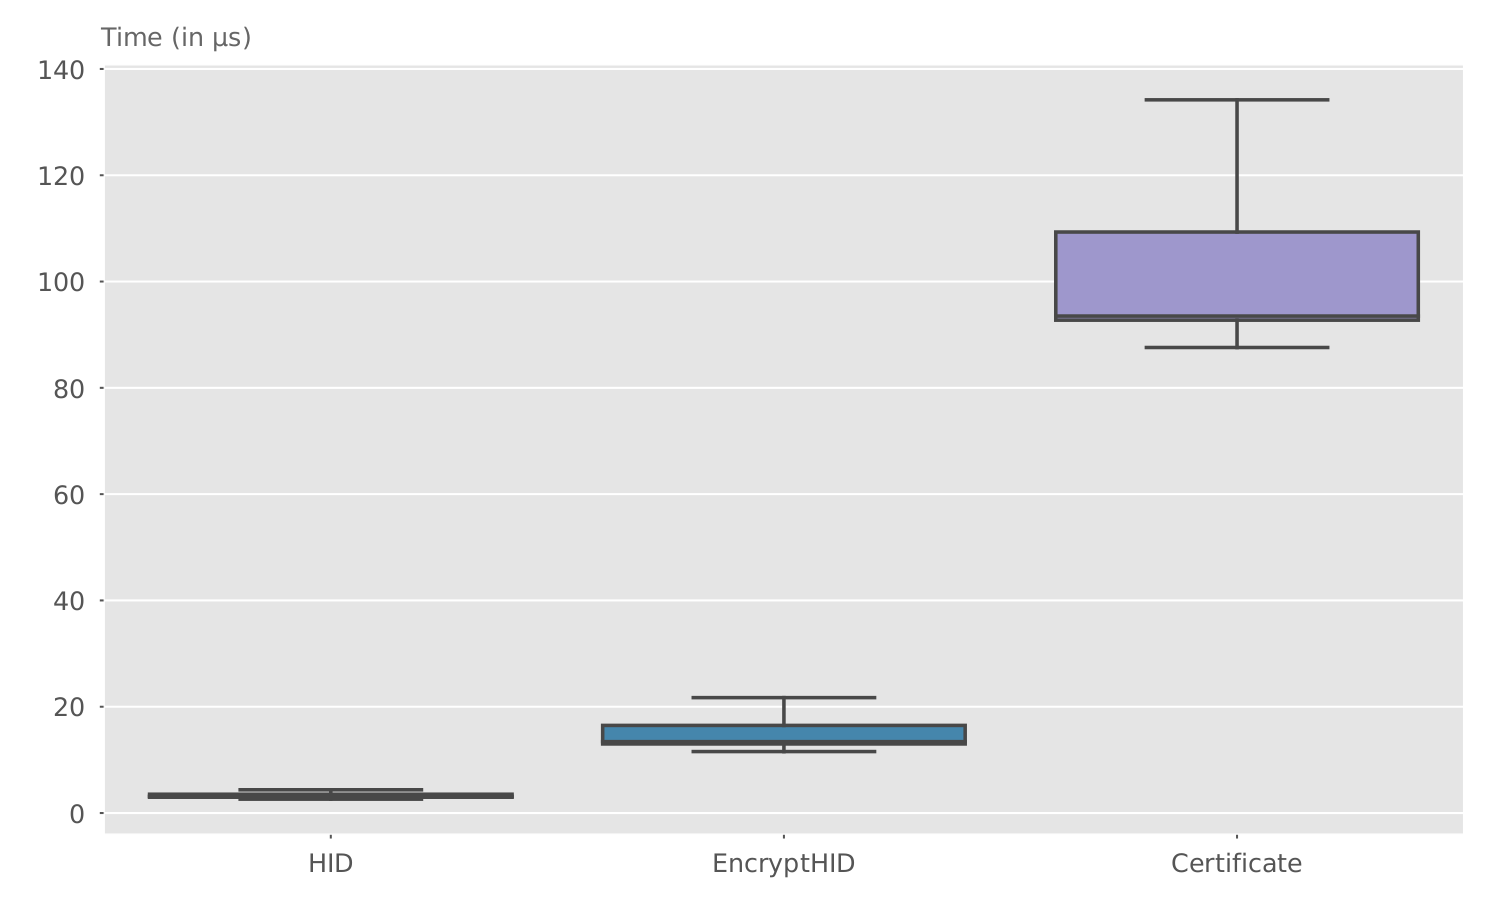
\includegraphics[scale=0.3]{Figures/ephid_gen_stat.png}}
\decoRule
\caption[EphID Generation Ops]{Time taken by different operation involved in EphID generation}
\label{fig:perf_ephid}
\end{figure}

\section{DNS}
\begin{figure}[th!!]
\centering
\noindent
\makebox[\textwidth]{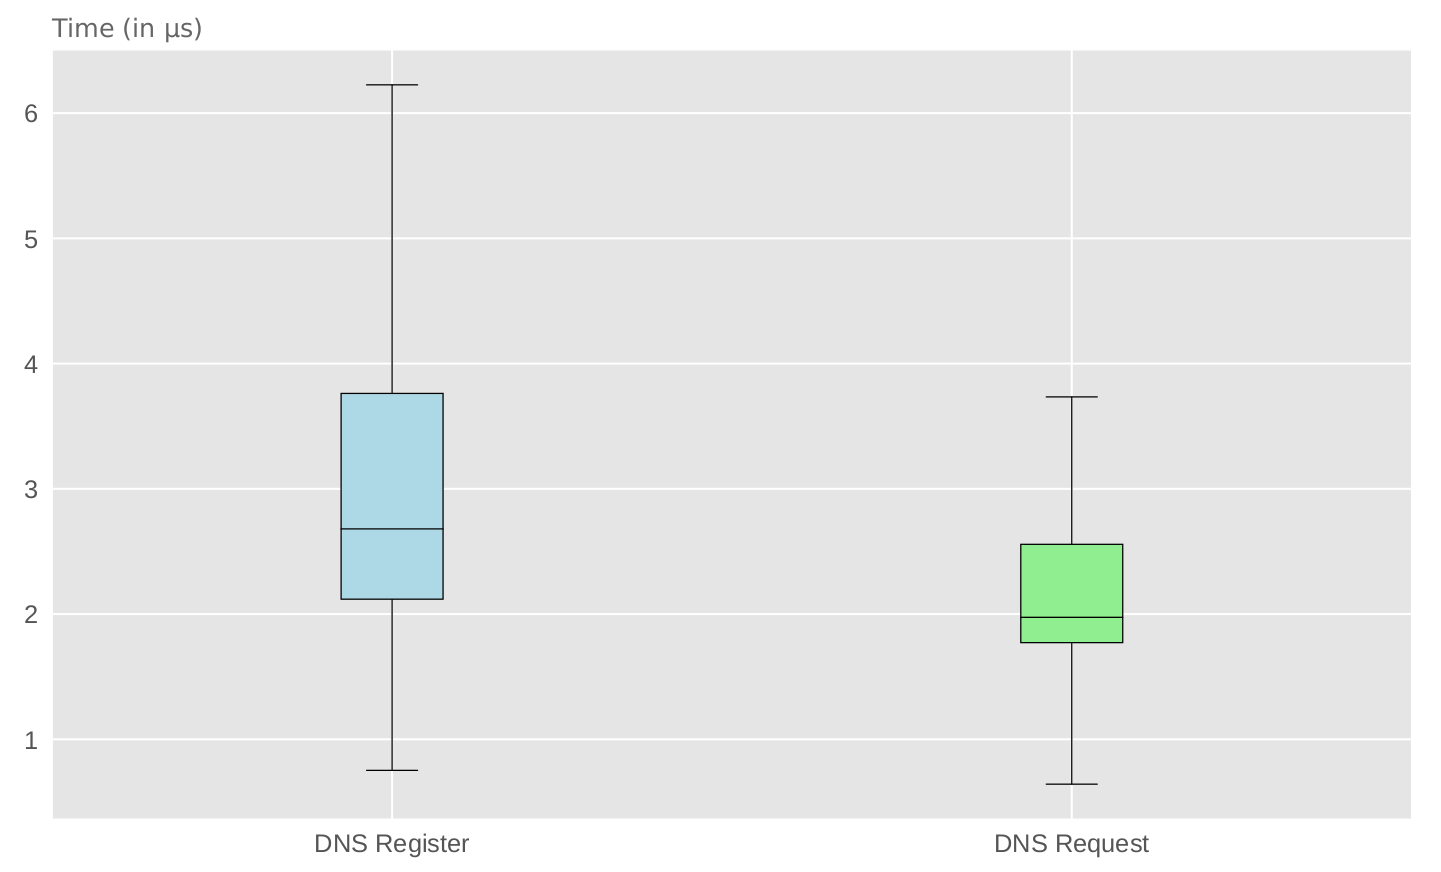
\includegraphics[scale=0.3]{Figures/dns_bench.png}}
\decoRule
\caption[DNS Operations]{Time taken by APNA MS for DNS Register and Request}
\label{fig:perf_ephid}
\end{figure}

\section{MACKey}
\begin{figure}[th!!]
\centering
\noindent
\makebox[\textwidth]{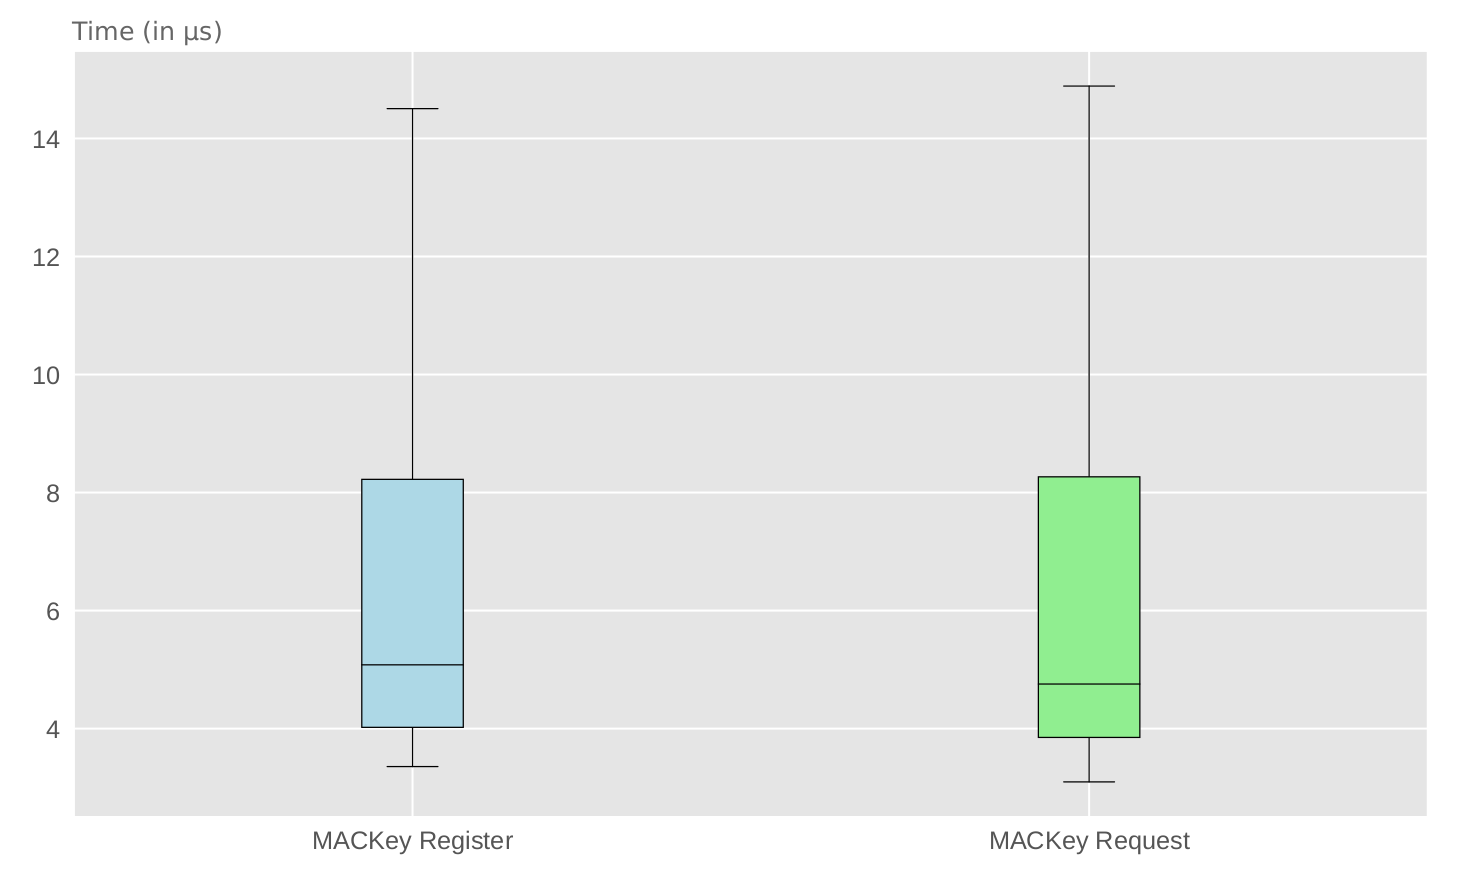
\includegraphics[scale=0.3]{Figures/mac_bench.png}}
\decoRule
\caption[MACKey Operations]{Time taken by APNA MS for MACKey Register and Request}
\label{fig:perf_ephid}
\end{figure}

\section{Host ID}
\begin{figure}[th!!]
\centering
\noindent
\makebox[\textwidth]{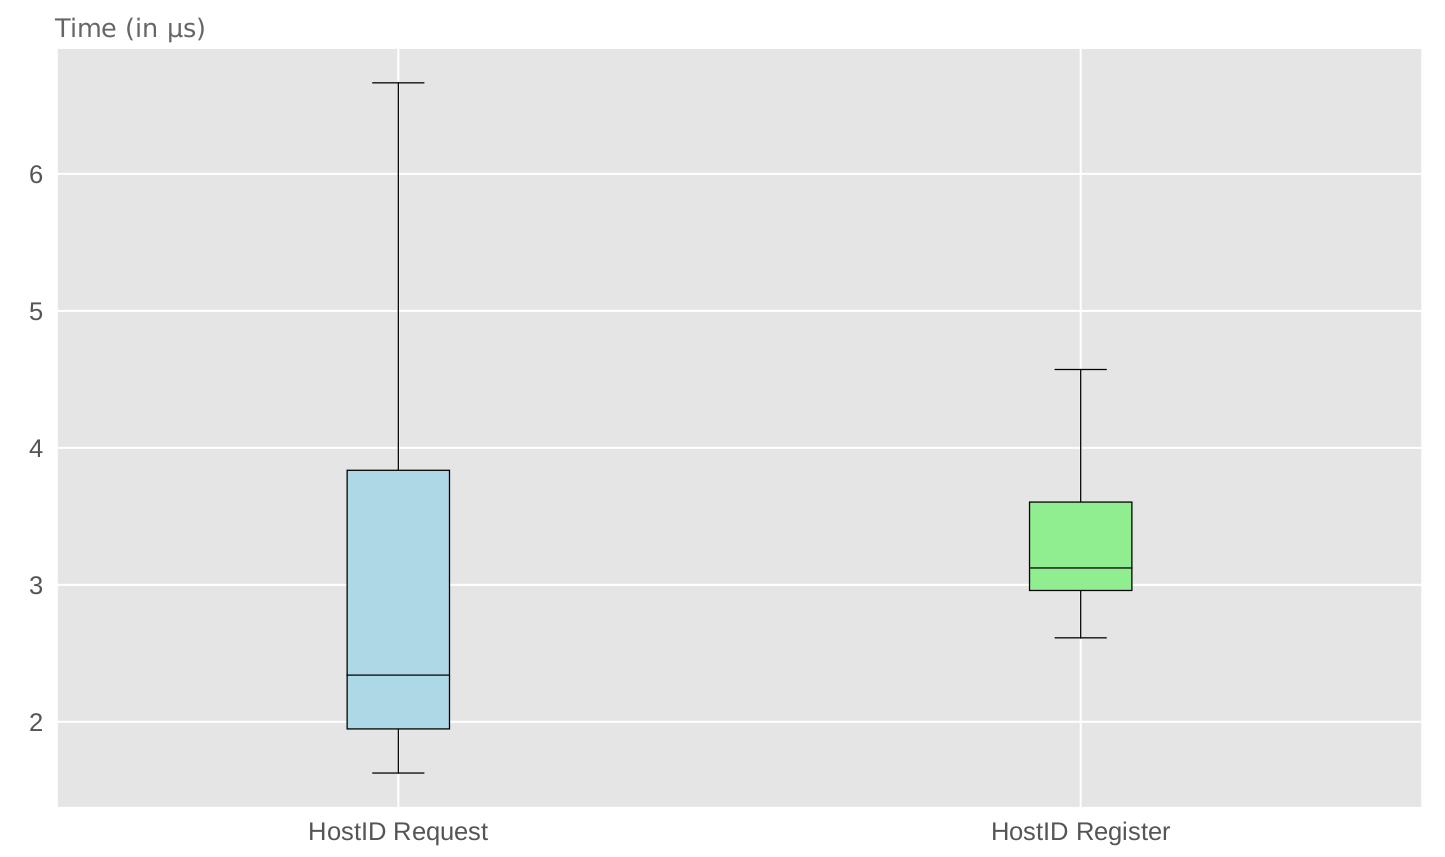
\includegraphics[scale=0.3]{Figures/hid_bench.png}}
\decoRule
\caption[HostID Operations]{Time taken by APNA MS for HostID Register and Request}
\label{fig:perf_ephid}
\end{figure}

\section{Latency}
\begin{figure}[th!!]
\centering
\noindent
\makebox[\textwidth]{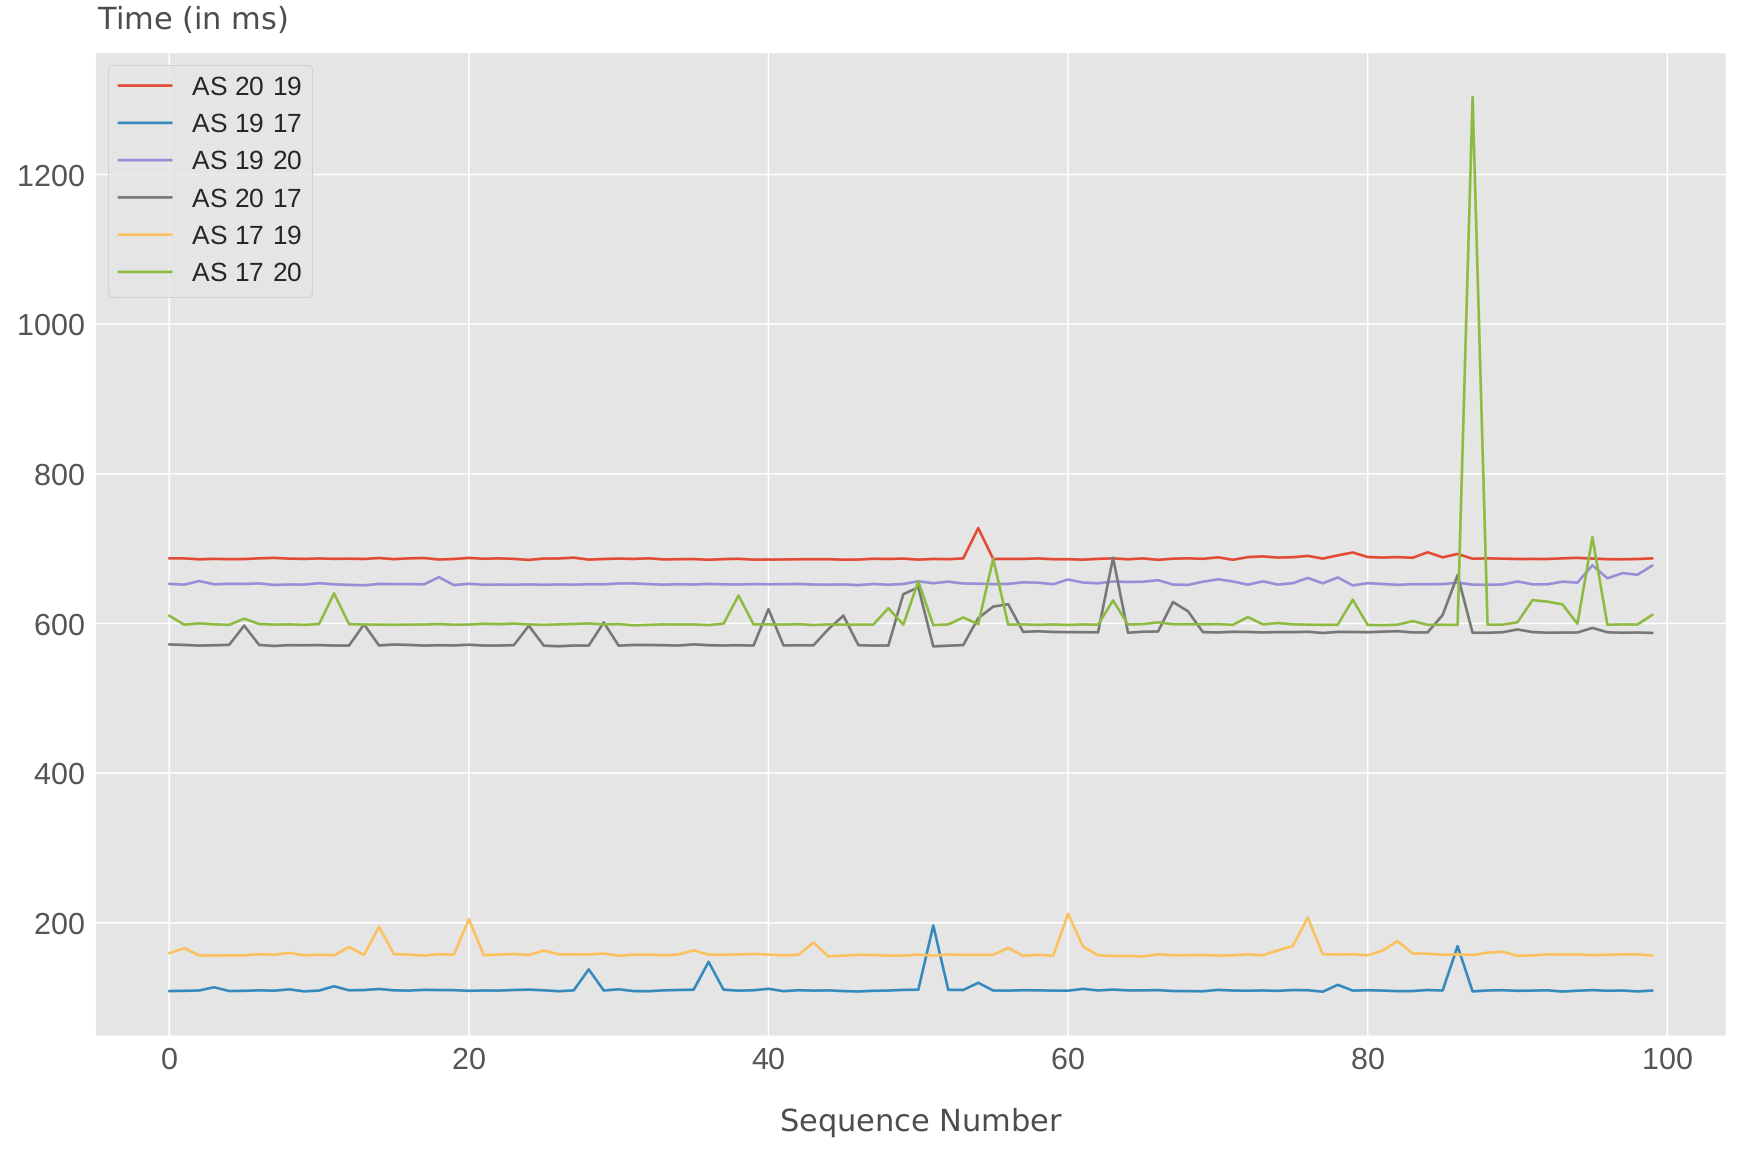
\includegraphics[scale=0.3]{Figures/vanilla_scion_lat.png}}
\decoRule
\caption[Latency Analysis]{Latency Analysis for Vanilla SCION}
\label{fig:perf_ephid}
\end{figure}